\renewcommand{\theequation}{\theenumi}
\begin{enumerate}[label=\arabic*.,ref=\thesubsection.\theenumi]
\numberwithin{equation}{enumi}
\item 
\begin{align}
\begin{bmatrix}x & y\end{bmatrix}\begin{bmatrix}A & \frac{B}{2}\\\frac{B}{2} & C\end{bmatrix}\begin{bmatrix}x \\ y\end{bmatrix} + \begin{bmatrix}D & E\end{bmatrix}\begin{bmatrix}x & y\end{bmatrix} +k
\end{align}

\item
\begin{align}
\begin{bmatrix}\vec x\end{bmatrix}^T\begin{bmatrix}1 & 0\\0 & 0\end{bmatrix}\begin{bmatrix}\vec x\end{bmatrix} + \begin{bmatrix}-2 & 0\end{bmatrix}\begin{bmatrix}\vec x\end{bmatrix} -8
\\
Ax^2+Cy^2+Bxy+Dx+Ey+k
\\
Ax^2+Dx-8 = 0
\\
x^2-2x-8 = 0
\end{align}
\begin{align}
s_1 =  \frac{-D + \sqrt{D^2 - 4\times A\times 8 }}{2\times A}
\\
=  \frac{-D + \sqrt{D^2 + 32\times A }}{2\times A} = 4 
\\
s_2 =  \frac{-D - \sqrt{D^2 - 4\times A\times 8 }}{2\times A}
\\
\frac{-D - \sqrt{D^2 + 32\times A }}{2\times A} = -2
\end{align}
\begin{figure}[!ht]
	\centering
	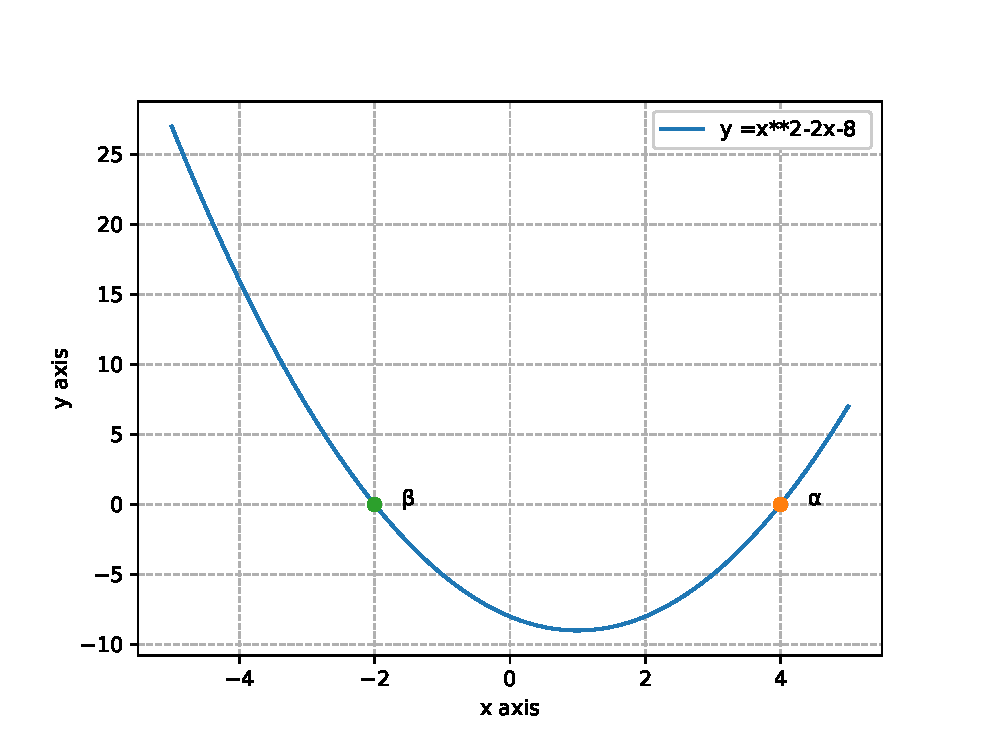
\includegraphics[width=\columnwidth]{./figures/conics/perabola1.eps}
	\caption{equation 1 }
	\label{fig:perabola1}
\end{figure}
\begin{lstlisting}
codes/conics/perabola2.py
\end{lstlisting}


\item
\begin{align}
\begin{bmatrix}\vec x\end{bmatrix}^T\begin{bmatrix}4 & 0\\0 & 0\end{bmatrix}\begin{bmatrix}\vec x\end{bmatrix} + \begin{bmatrix}8 & 0\end{bmatrix}\begin{bmatrix}\vec x\end{bmatrix} 
\\
Au^2+Cv^2+Buv+Du+Ev+k =0
\\
Au^2+Du = 0
\\
4u^2 + 8u = 0
\\
u_1 =  \frac{-D + \sqrt{D^2 - 4\times A\times 8 }}{2\times A}
\\
=  \frac{-D + D}{2\times A} = 0
\\
u_2 =  \frac{-D - \sqrt{D^2 - 4\times A\times 8 }}{2\times A}
\\
\frac{-D }{A} = -2
\end{align}
\begin{figure}[!ht]
	\centering
	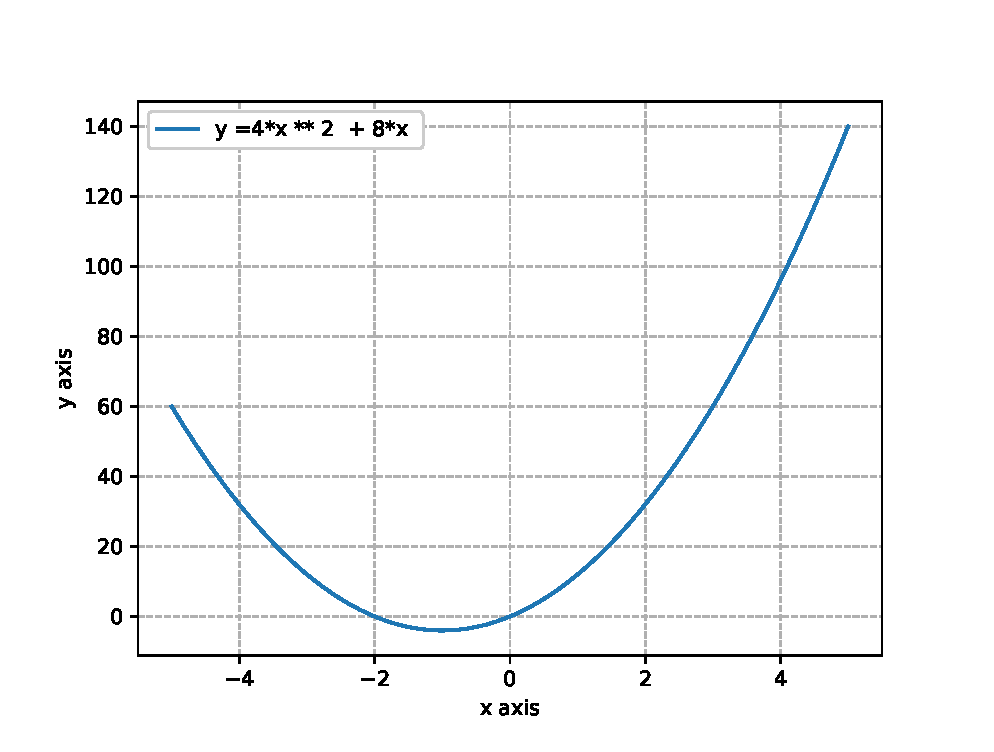
\includegraphics[width=\columnwidth]{./figures/conics/perabola2.eps}
	\caption{equation 2 }
	\label{fig:perabola2}
\end{figure}
\begin{lstlisting}
codes/conics/perabola2.py
\end{lstlisting} 

\item
\begin{align}
\begin{bmatrix}\vec x\end{bmatrix}^T\begin{bmatrix}4 & 0\\0 & 0\end{bmatrix}\begin{bmatrix}\vec x\end{bmatrix} + \begin{bmatrix}-4 & 0\end{bmatrix}\begin{bmatrix}\vec x\end{bmatrix} +1
\\
Ax^2+Cy^2+Bxy+Dx+Ey+k =0
\\
Ax^2+Dx + 1 = 0
\\
4x^2-4x+1 = 0
\\
s_1 =  \frac{-D + \sqrt{D^2 + 4\times A }}{2\times A} = \frac{1}{2}
\\
s_2 =  \frac{-D - \sqrt{D^2 +4\times A }}{2\times A} = -\frac{1}{2}
\end{align}
\begin{figure}[!ht]
	\centering
	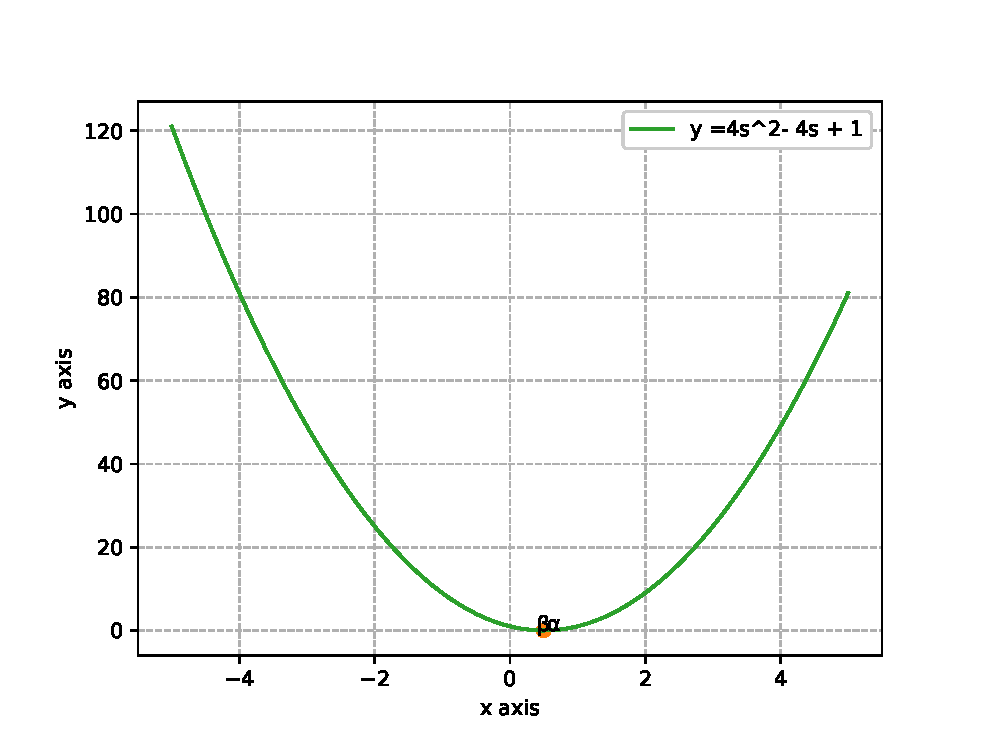
\includegraphics[width=\columnwidth]{./figures/conics/perabola3.eps}
	\caption{equation 3 }
	\label{fig:perabola3}
\end{figure}
\begin{lstlisting}
codes/conics/perabola3.py
\end{lstlisting}

\item
\begin{align}
\begin{bmatrix}\vec x\end{bmatrix}^T\begin{bmatrix}1 & 0\\0 & 0\end{bmatrix}\begin{bmatrix}\vec x\end{bmatrix} + \begin{bmatrix}0 & 0\end{bmatrix}\begin{bmatrix}\vec x\end{bmatrix} -15
\\
Ax^2+Cy^2+Bxy+Dx+Ey+k =0
\\
At^2 - 15= 0
\\
t^2 - 15 = 0
\\
s_1 =  \frac{-D + \sqrt{D^2 + 4\times A\times 15 }}{2\times A}
\\
=  \frac{ \sqrt{60\times A }}{2\times A} = \sqrt {15}
\\
s_2 =  \frac{-D - \sqrt{D^2 + 4\times A\times 15 }}{2\times A}
\\
\frac{ - \sqrt{ 60\times A }}{2\times A} = -\sqrt {15}
\end{align}
\begin{figure}[!ht]
	\centering
	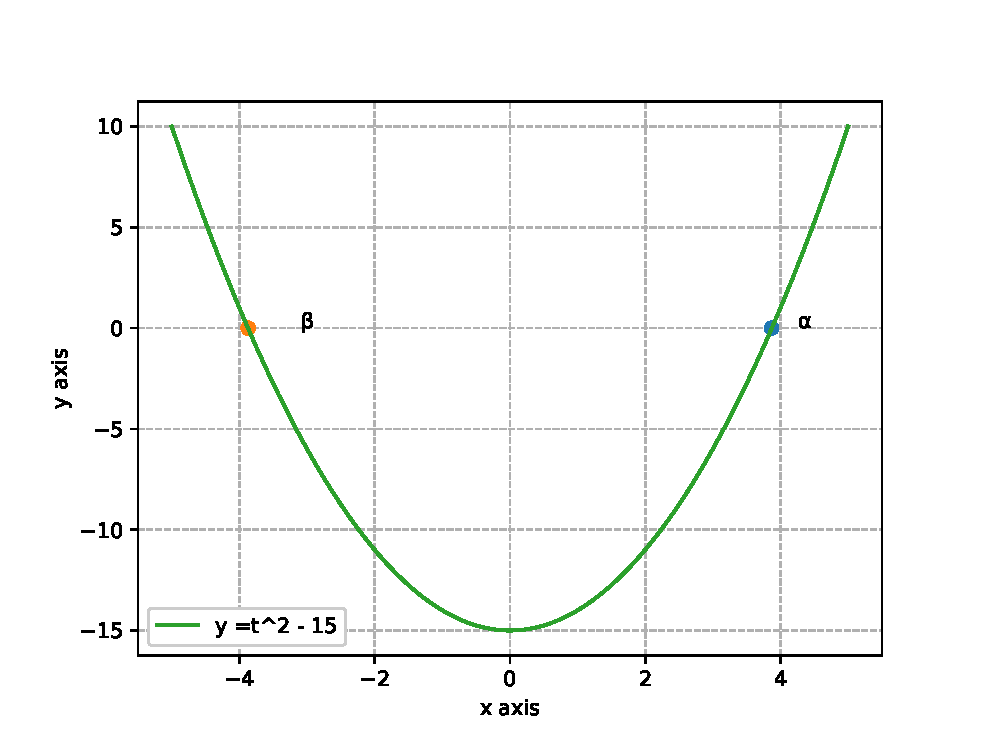
\includegraphics[width=\columnwidth]{./figures/conics/perabola4.eps}
	\caption{equation 4 }
	\label{fig:perabola4}
\end{figure}
\begin{lstlisting}
codes/conics/perabola4.py
\end{lstlisting}

\item
\begin{align}
\begin{bmatrix}\vec x\end{bmatrix}^T\begin{bmatrix}6 & 0\\0 & 0\end{bmatrix}\begin{bmatrix}\vec x\end{bmatrix} + \begin{bmatrix}-7 & 0\end{bmatrix}\begin{bmatrix}\vec x\end{bmatrix} -3
\\
Ax^2+Cy^2+Bxy+Dx+Ey+k =0
\\
Ax^2 + Dx- 3= 0
\\
6x^2-3-7x = 0
\\
x_1 =  \frac{-D + \sqrt{D^2 + 4\times A\times 3 }}{2\times A}
\\
=  \frac{-D + \sqrt{D^2 - 12\times A }}{2\times A} = \frac{3}{2}
\\
x_2 =\frac{-D - \sqrt{D^2 - 12\times A }}{2\times A} = -\frac{1}{3} 
\end{align}
\begin{align}
x_2 =\frac{-D - \sqrt{D^2 - 12\times A }}{2\times A} = -\frac{1}{3}
\end{align}
\begin{figure}[!ht]
	\centering
	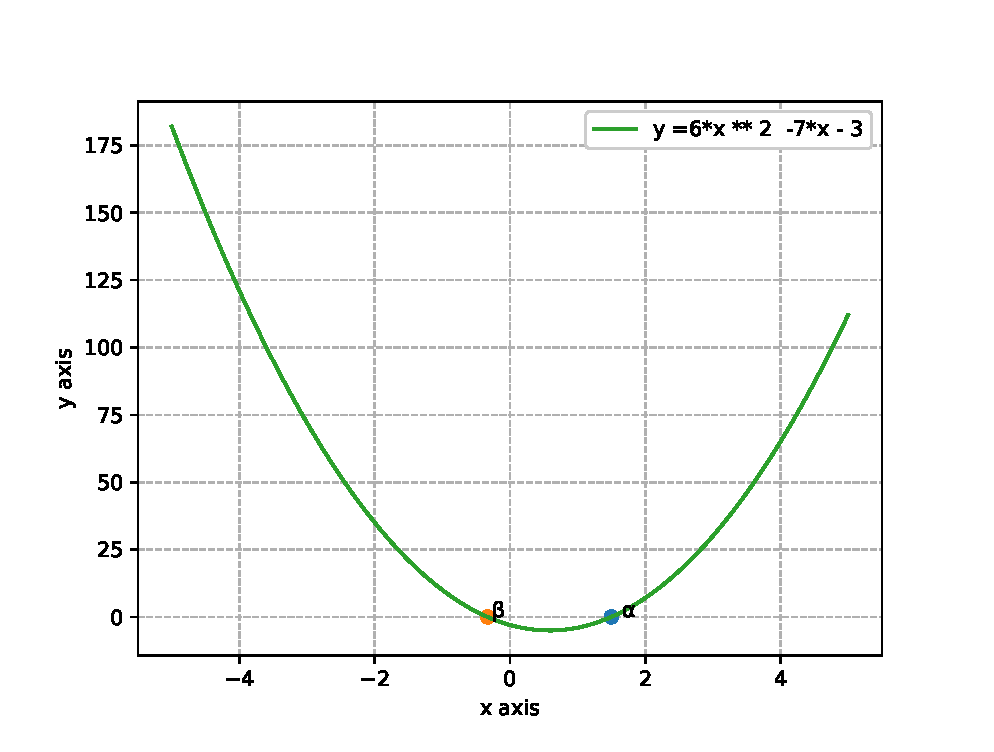
\includegraphics[width=\columnwidth]{./figures/conics/perabola5.eps}
	\caption{equation 5 }
	\label{fig:perabola5}
\end{figure}
\begin{lstlisting}
codes/conics/perabola5.py
\end{lstlisting}

\item
\begin{align}
\begin{bmatrix}\vec x\end{bmatrix}^T\begin{bmatrix}3 & 0\\0 & 0\end{bmatrix}\begin{bmatrix}\vec x\end{bmatrix} + \begin{bmatrix}-1 & 0\end{bmatrix}\begin{bmatrix}\vec x\end{bmatrix} -4
\\
Ax^2+Cy^2+Bxy+Dx+Ey+k =0
\\
Ax^2 + Dx-8= 0
\\
3x^2-2x-8= 0
\\
x_1 =  \frac{-D + \sqrt{D^2 - 32\times A }}{2\times A} =  -1
\\
x_2 =\frac{-D + \sqrt{D^2 - 12\times A }}{2\times A} = -\frac{4}{3}
\end{align}
\begin{figure}[!ht]
	\centering
	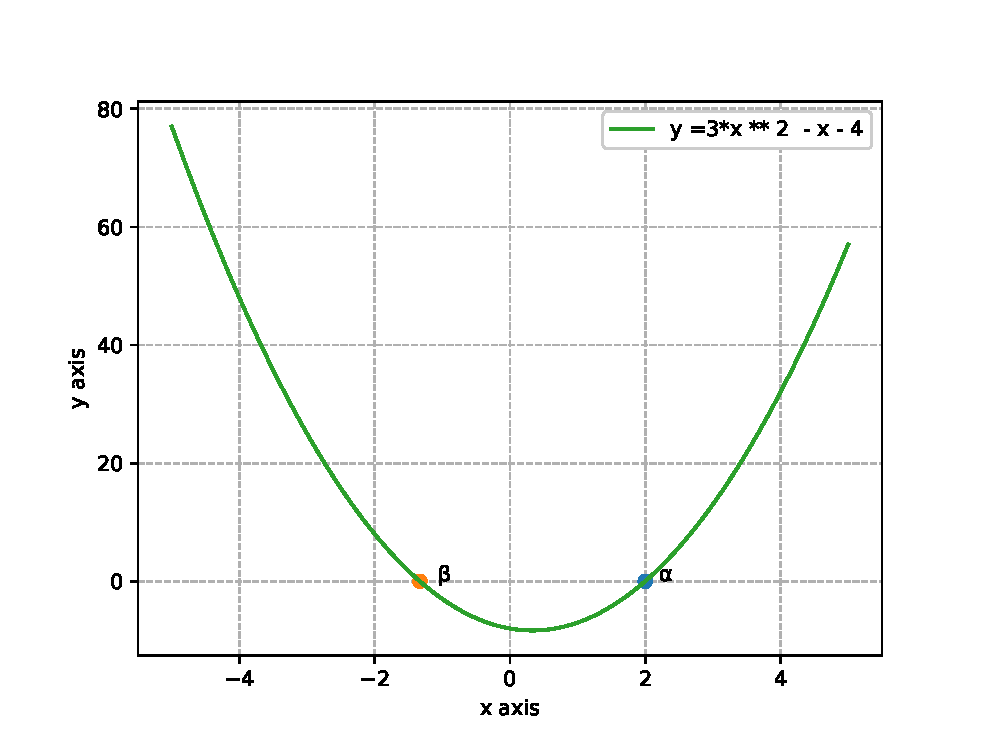
\includegraphics[width=\columnwidth]{./figures/conics/perabola6.eps}
	\caption{equation 6 }
	\label{fig:perabola6}
\end{figure}
  
\begin{lstlisting}
codes/conis/perabola6.py
\end{lstlisting}
Path for python code for the figure is as above
\end{enumerate}